\newpage
%%%%%%%%%%%%%%
\section{Evaluaci\' on}
%%%%%%%%%%%%%%

\par Para evaluar las pruebas planteadas en el apartado anterior, se ejecutaron los bancos de pruebas y se graficaron las se\~ nales resultantes (archivo signals.vcd), para analizar los resultados obtenidos.
\\
\par En los siguientes apartados se muestran los resultados obtenidos para cada uno de los multiplicadores.

\subsection{Banco de pruebas del decodificador de instrucciones}
El decodificador de instrucciones es el m\' odulo que se encarga de ajustar todas las se\~ nales de control del procesador de acuerdo a la instrucci\' on que se est\' a procesando en cada ciclo de reloj, de manera tal que debe ser capaz de obtener la decodificaci\' on de la instrucci\' on, las se\~ nales de control: \textit{write to a, write to b, mux pre alu a, mux pre alu b, read write, write back mux, jump, write mux y branch taken} de acuerdo al avance del contador de programa \textit{pc}.

Es de esta manera como se realiz\' o la simulaci\' on de las instrucciones que modifican las se\~ nales de control y se puede observar en la Figura \ref{fig:decoder} como efectivamente se tienen los resultados esperados de acuerdo con el dise\~ no del procesador.

\begin{figure}[hbtp]
\caption{Simulaci\' on del decodificador de instrucciones}
\centering
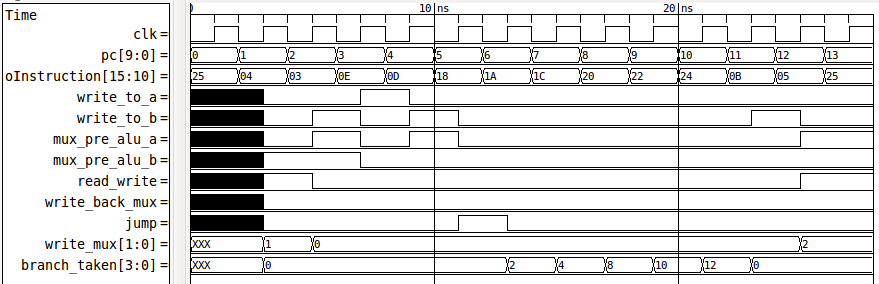
\includegraphics[scale=0.6]{../Codes/Verilog_Testbenches/scopes/Decoder_scope.png}
\label{fig:decoder}
\end{figure}


\subsection{Banco de pruebas de la ALU}
El m\' odulo ALU es el que se encarga de realizar el c\' alculo aritm\' etico de ciertas instrucciones que lo requieren y adem\' as obtener el valor de la se\~ nal de carry y la se\~ nal de cero. Tambien se encarga de realizar el c\' alculo de las direcciones de memoria para instrucciones que tienen que ver con el acceso o ingreso a la memoria principal.

De acuerdo con lo anterior y con la descripci\' on proporcionada en la secci\' on de dise\~ no se puede observar los resultados de la simulaci\' on efectuada en la Figura \ref{fig:alu} donde cabe destacar que el valor de los operandos \textit{in1, in2} y el resultado final \textit{out} se observa en formato decimal, mientras que las se\~ nales de \textit{carry} y \textit{zero} son bits.


\begin{figure}[hbtp]
\caption{Simulaci\' on de m\' odulo alu}
\centering
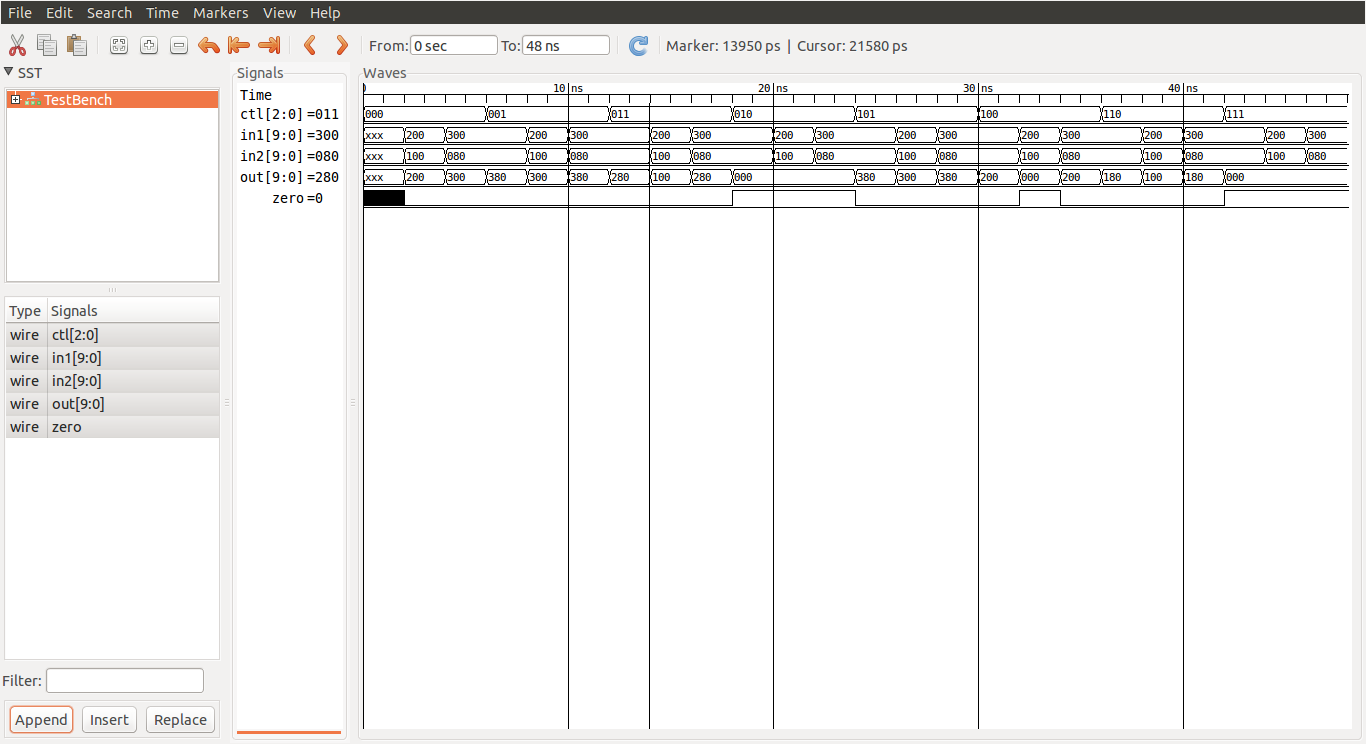
\includegraphics[scale=0.48]{../Codes/Verilog_Testbenches/scopes/ALU.png}
\label{fig:alu}
\end{figure}

\subsection{Banco de pruebas del controlador de ALU}
El m\' odulo controlador de la ALU es bastante importante en tanto que se encarga de obtener los bits de control que se encargan de decirle al m\' odulo ALU la tarea que debe desarrollar, por lo que en la evaluaci\' on de este m\' odulo se debe de tener como entrada todas las posibles instrucciones que se pueden ejecutar en el procesador y obtener a partir del c\' odigo de instrucci\' on, el c\' odigo de operando que debe implementar la ALU.

El resultado de la simulaci\' on se puede observar en la Figura \ref{fig:aluControl} donde se puede destacar que los c\' odigos de presentan en formato octal y adem\' as en orden de acuerdo con la descripci\' on presentada en la secci\' on de dise\~ no.

\begin{figure}[hbtp]
\caption{Simulaci\' on de m\' odulo controlador de alu}
\centering
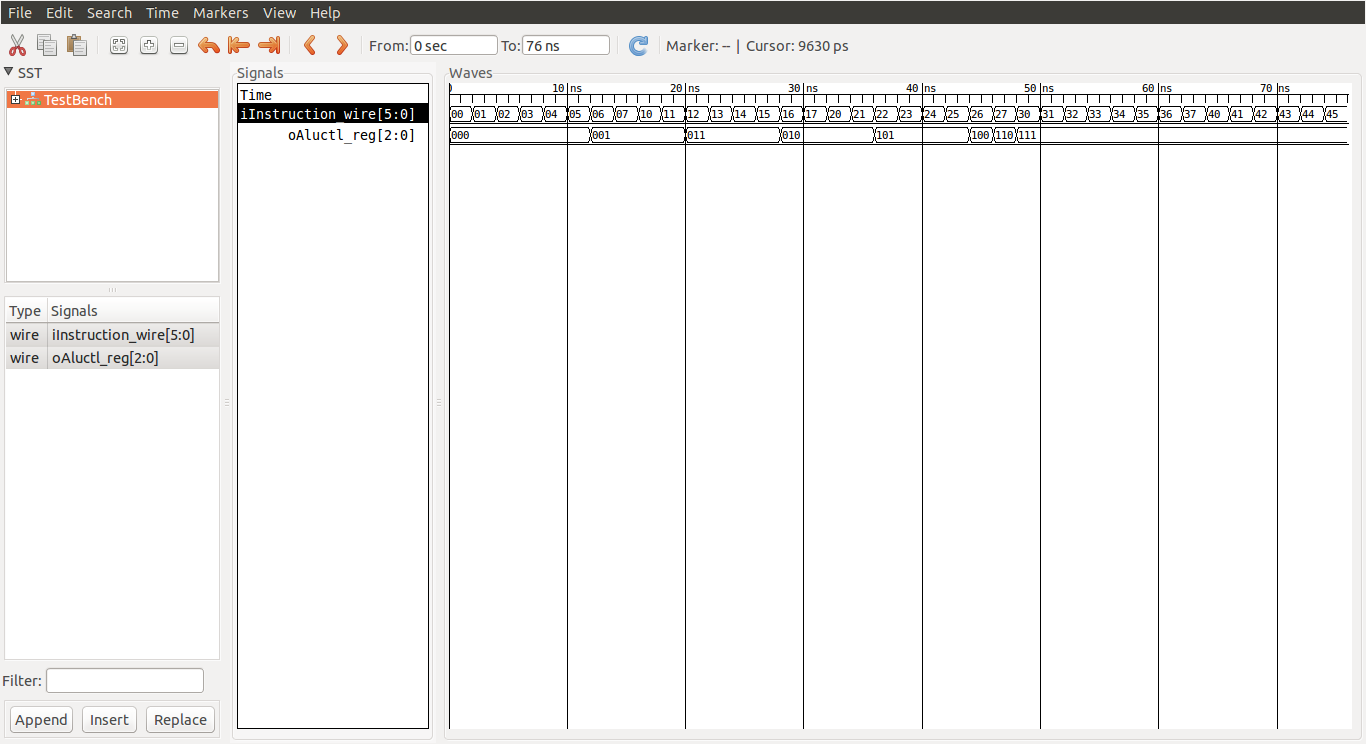
\includegraphics[scale=0.48]{../Codes/Verilog_Testbenches/scopes/ALU_Controller_scope.png}
\label{fig:aluControl}
\end{figure}


\subsection{Banco de pruebas del m\' odulo \textit{branch\_taken}}
El m\'odulo \textit{branch\_taken} se encarga de revisar cual branch se desea tomar y si se cumplen las condiciones para tomarlo, esto por medio de los bits de status especificados: $C_{A}$, $N_{A}$, $Z_{A}$, $C_{B}$, $N_{B}$, $Z_{B}$.\\

En la tabla \ref{t:saltos} se muestran los valores asociados a cada uno de los saltos relativos (branches) definidos, as\'i como la condici\'on que permite que estos sea tomados. Basado en esta tabla, se escribi\'o un banco de pruebas con el objetivo de probar el correcto funcionamiento del m\'odulo, los resultados obtenidos de la ejecuci\'on de este banco de pruebas se muestran en la figura \ref{f:branch_taken_results}.\\

\begin{table}[h!]
\centering
\caption{Saltos relativos y condiciones para ser tomados}
\label{t:saltos}
\begin{tabular}{|c|c|c|}
\hline
{\bf Branch} & {\bf Valor} & {\bf Condici\'on para ser tomado} \\ \hline
BAEQ         & $1$         & $Z_{A}$ $=$ $1$                   \\ \hline
BANE         & $2$         & $Z_{A}$ $=$ $0$                   \\ \hline
BACS         & $3$         & $C_{A}$ $=$ $1$                   \\ \hline
BACC         & $4$         & $C_{A}$ $=$ $0$                   \\ \hline
BAMI         & $5$         & $N_{A}$ $=$ $1$                   \\ \hline
BAPL         & $6$         & $N_{A}$ $=$ $0$                   \\ \hline
BBEQ         & $7$         & $Z_{B}$ $=$ $1$                   \\ \hline
BBNE         & $8$         & $Z_{B}$ $=$ $0$                   \\ \hline
BBCS         & $9$         & $C_{B}$ $=$ $1$                   \\ \hline
BBCC         & $10$        & $C_{B}$ $=$ $0$                   \\ \hline
BBMI         & $11$        & $N_{B}$ $=$ $1$                   \\ \hline
BBPL         & $12$        & $N_{B}$ $=$ $0$                   \\ \hline
\end{tabular}
\end{table}

\begin{figure}[hbtp]
\caption{Simulaci\' on del m\'odulo \textit{branch\_taken}}
\centering
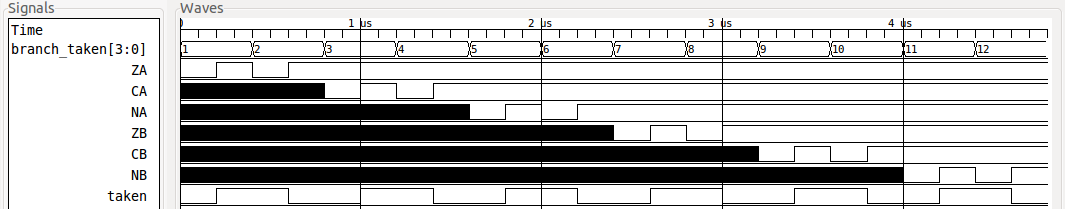
\includegraphics[scale=0.48]{../Codes/Verilog_Testbenches/scopes/branch_taken.png}
\label{f:branch_taken_results}
\end{figure}

En la figura \ref{f:branch_taken_results}, se puede notar que los saltos relativos definidos por la se\~nal \textit{branch\_taken[3:0]}, se est\'an tomando, es decir la se\~nal \textit{taken} est\'a en $1$, cuando se cumple la condici\'on necesaria dada por las se\~nales \textit{ZA}, \textit{CA}, \textit{NA}, \textit{ZB}, \textit{CB} y \textit{NB}, con lo que se puede concluir que el m\'odulo tiene el funcionamiento esperado.\\

\subsection{Banco de pruebas del m\' odulo \textit{branch\_calc}}
El m\'odulo \textit{branch\_calc} se encarga de calcular el nuevo valor del contador del programa si el salto relativo debe ser tomado. Se espera que el m\'odulo sume o reste, seg\'un el valor de s\'etimo bit de la instrucci\'on $0$ u $1$ respectivamente, al valor del contador de programa el valor indicado en la instrucci\'on.\\

Para probar el adecuado funcionamiento de este m\'odulo se escribi\'o un banco de pruebas en el que se probaron diferentes valores de la constante que acompa\~na a la instrucci\'on, buscando probar casos con el s\'etimo bit de la instrucci\'on en $1$ y en $0$.\\

En la figura \ref{f:branch_calc_results} se muestran los resultados tras la ejecuci\'on de dicho banco de pruebas, donde se puede ver que efectivamente a la se\~nal \textit{pc\_in} que se defini\'o con un valor de $100$ se le suma el valor del salto (se\~nal \textit{value\_branch}) cuando el s\'etimo bit (se\~nal \textit{bit}) est\'a en $0$, ambas tomadas del valor de la se\~nal \textit{const}, y se resta cuando el s\'etimo bit est\'a en $1$.\\

De forma que se puede concluir que el m\'odulo cumple adecuadamente con sus especificaciones.\\

\begin{figure}[hbtp]
\caption{Simulaci\' on del m\'odulo \textit{branch\_calc}}
\centering
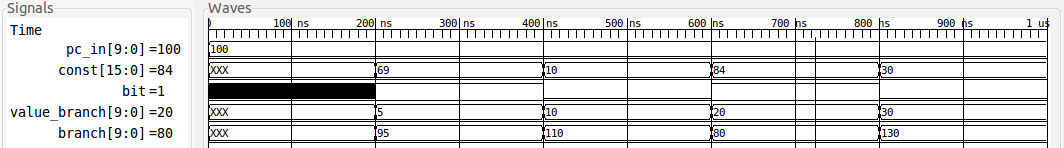
\includegraphics[scale=0.48]{../Codes/Verilog_Testbenches/scopes/branch_calc.png}
\label{f:branch_calc_results}
\end{figure}

\subsection{Banco de pruebas de los saltos relativos (branches)}

Para comprobar que los saltos relativos (branches) se ejecutan de la forma correcta se escribi\'o una secuencia de instrucciones, en la cual se cre\'o un lazo utilizando el branch $BANE$ ($1A$), el cual se ejecuta si se cumple que $Z_{A}$ $=$ $0$, es decir si el registro A tiene un valor distinto a cero.\\

En la figura \ref{f:branches_scope} se muestran los resultados obtenidos al ejecutar dicha secuencia, se puede ver que una vez que el branch ingresa, pasan dos ciclos de reloj para que la instrucci\'on llegue a $MEM$ y posteriormente es ejecutado seg\'un los valores especificados en las instrucciones. En este caso, el valor del salto es de 5, de forma que el program counter se devuelve a la instrucci\'on $STB$ ($05$) en la secuencia de instrucciones.\\

Con esto se concluye que efectivamente los saltos relativos tienen el comportamiento esperado.\\

\begin{figure}[hbtp]
\caption{Evaluaci\'on de los saltos relativos}
\centering
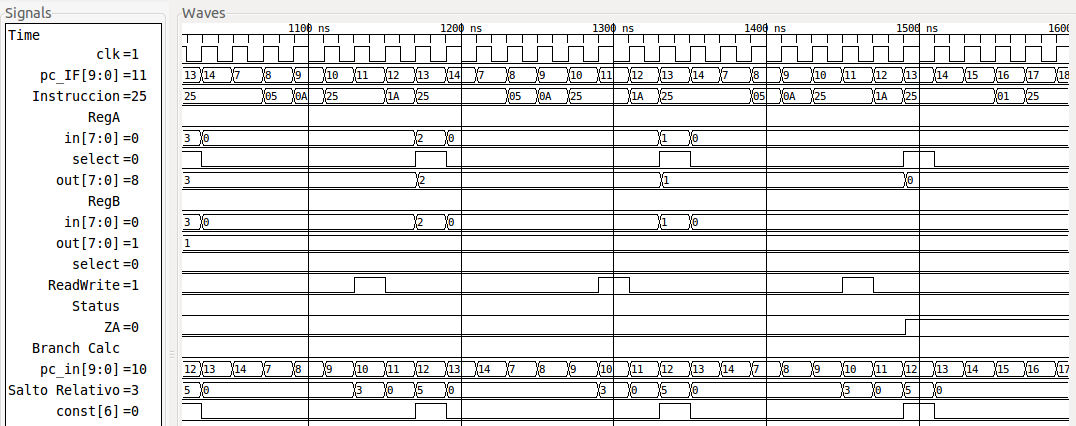
\includegraphics[scale=0.45]{../Codes/Verilog_Testbenches/scopes/Branches.png}
\label{f:branches_scope}
\end{figure}



\subsection{Banco de pruebas de las memorias}
Se realiz\' o una evaluaci\' on de la memoria RAM tal com se puede observar en la Figura \ref{fig:RAMmem} en donde se realizan 1024 iteraciones de escritura a la memoria para que tenga valores almacenados, y luego se realizan 1024 lecturas a todas las posiciones de memoria. En la Figura \ref{fig:RAMmem} se muestra donde hace el cambio de escritura a lectura para mostrar el comportamiento de las dos posibles acciones que se pueden llevar a cabo en este m\' odulo.

\begin{figure}[hbtp]
\caption{Evaluaci\' on de la memoria RAM}
\centering
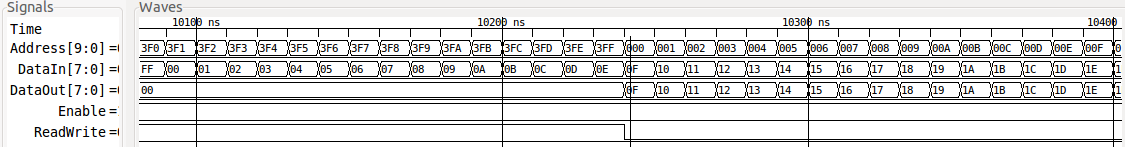
\includegraphics[scale=0.45]{../Codes/Verilog_Testbenches/scopes/RamScope.png}
\label{fig:RAMmem}
\end{figure}



\subsection{Banco de pruebas de la unidad de forwarding}
La unidad de \textit{forwarding o bypassing} es un m\' odulo bastante separado del resto del pipeline y b\' asicamente se agrega como una mejora al dise\~ no ya funcional con el fin de mejorar el desempe\~ no de ciertos programas que ejecutan instrucciones de manera tal que producen alertas o \textit{hazards} en el funcionamiento.

Se realiz\' o una prueba a este m\' odulo en donde se ejecute una secuencia de instrucciones para tratar de comprobrar que se afecta un registro una o m\' as veces consecutivas. En t\' erminos generales se puede observar en la Figura \ref{fig:forwarding} que primero viene una instrucci\' on que afecta el registro A, luego una instrucci\' on que no lo afecta. Luego se tienen dos instrucciones seguidas que afectan al registro A y finalmente tres instrucciones seguidas que afectan el registro A.

La secuencia de instrucciones implementada es tal que en principio debe comprobrar todos lo posibles casos, tal como se describe el comienzo de las instrucciones a continuaci\' on: 

\begin{itemize}
\item  ADDA: Se tiene una instrucc\' ion de suma sin dependencias por lo cual no levanta ninguna de las se\~ nales de control.
\item LDA: No hay dependencias por lo tanto no levanta ninguna se\~ nal de control.
\item NOP: No hace nada. No levanta ninguna se\~ nal de control. Aparece 3 veces seguidas.
\item LDCA: No tiene dependencia con ninguna instrucci\' on. No levanta ninguna se\~ nal de control.
\item LDCB: No tiene dependencia con ninguna instrucci\' on. No levanta ninguna se\~ nal de control.	 	
\item ORB: Tiene una dependencia directa con la instrucci\' on anterior, por lo tanto debe activar la se\~ nal de control outputB EX, porque el operando se encuentra actualizado en el registro EX MEM. Adem\' as con la instrucci\' on transanterior por lo que debe activar la se\~ nal outputA MEM, ya que el operando actual se encuentra actualizado en MEM WB
\item ADDB: Es una dependencia directa con la instrucc\' ion anterior, por lo que debe activar la se\~ nal de control outputB MEM y la transanterior con outputB EX
\item SUBA: Tiene una dependencia directa con la instrucci\' on anterior y la transanterior por eso se levantan las dos se\~ nales de control correspondientes.
\item NOP dos veces. No hace nada por lo tanto no activa ninguna se\~ nal de control.
\item ANDA. No posee dependencia pues la NOP anterior se ejecuta dos veces y elimina el problema de la posible dependencia.
\item NOP. No hace nada por lo tanto no activa ninguna se\~ nal de control.
\item SUBA. Esta instrucci\' on posee dependencia con la instrucci\' on del ciclo transanterior, pero solo para uno de los registros, por eso solo debe activar outputA MEM.
\item NOP. No hace nada por lo tanto no activa ninguna se\~ nal de control.
\item LDB. No posee dependencia pues hace lectura de memoria principal, por lo tanto no activa ninguna se\~ nal de control.
\end{itemize}	

\begin{comment}
\begin{itemize}
\item NOP: La primer instrucci\' on no ejecuta nada, no se levanta ninguna se\~ nal objetivo. (\textit{first A, first B, mux A, mux B}).
\item STA: No hay \textit{hazard} pues guarda en memoria lo que hay en el registro A. Levanta la se\~ nal \textit{first A} ya que se relaciona con el registro A.
\item LDCB: No hay \textit{hazard} pues no hay \textbf{dependiencias}. Levanta la se\~ nal \textit{first B} ya que se relaciona con el registro B. 
\item ANDA: No hay dependencia. Levanta \textit{first A}.
\item ADDA: Aparece la primer dependencia inmediata con la instrucci\' on anterior por lo que la se\~ nal \textit{mux A} se levanta dando a entender al procesador que debe hacer \textit{bypassing} de los datos.
\item JMP: No hay dependencia. No levanta ninguna se\~ nal.
\item ASLA: No hay dependiencia. Levanta la se\~ nal \textit{first A.}
\item LDA: \textbf{ESTA MALO, LEVANTA LA SENAL PERO NO DEBERIA}
\item SUBA: \textbf{CREO QUE ESTA MALO PORQUE HAY QUE METER UNA NOP} Hay una dependencia en tanto que la instrucci\' on anterior escribe en el registro A y la actual ocupa leer el contenido del registro A.
\item ADDB: No hay dependencia con las instrucciones anteriores. Adem\' as levanta la se\~ nal de control correspondiente \textit{first B}.
\item ANDB: Hay una dependencia directa con la instrucci\' on anterior en tanto que el valor que requiere como operando apenas est\' a en la salida de la ALU. Pero este caso lo resuelve bien ya que activa el \textit{mux B} y hace \textit{bypass} del valor correcto.
\item SUBB:  Hay una dependencia directa con la instrucci\' on anterior en tanto que el valor que requiere como operando apenas est\' a en la salida de la ALU. Pero este caso lo resuelve bien ya que activa el \textit{mux B} y hace \textit{bypass} del valor correcto.
\item STB:  Hay una dependencia directa con la instrucci\' on anterior en tanto que el valor que requiere como operando apenas est\' a en la salida de la ALU. Pero este caso lo resuelve bien ya que activa el \textit{mux B} y hace \textit{bypass} del valor correcto para almacenarlo en la memoria.
\item NOP: No realiza ninguna acci\' on por lo tanto no se levanta ninguna se\~ nal.
\end{itemize}
\end{comment}

Para mayor entendimiento se puede observar la definici\' on de las instrucciones en el ap\' endice \ref{apen1}

\begin{figure}[hbtp]
\caption{Evaluaci\' on del m\' odulo Forwarding Unit}
\centering
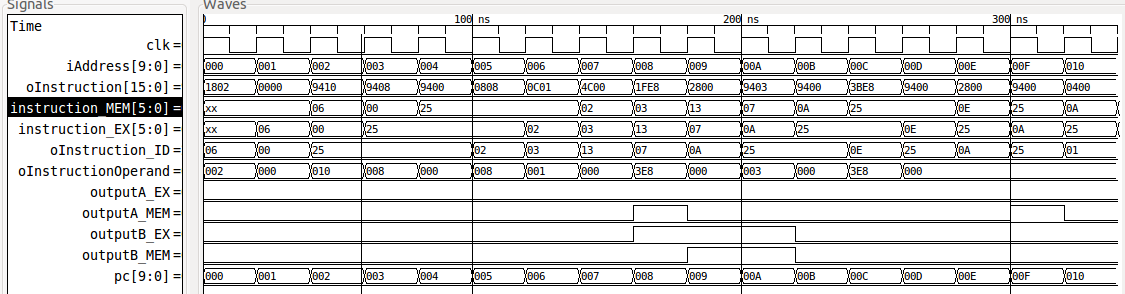
\includegraphics[scale=0.45]{../Codes/Verilog_Testbenches/scopes/Forwarding_unit.png}
\label{fig:forwarding}
\end{figure}



\subsection{Banco de pruebas de los registros}
Se realizaron pruebas al m\' odulo de los registro para comprobrar que efectivamente realizan lo esperado. Aunque en t\' erminos generales es un m\' odulo bastante peque\~ no en comparaci\' on con el resto de los m\' odulos, se defini\' o dentro de la estrategia de pruebas para evitar errores innecesarios a la hora de compilar, y pues el resultado obtenido se puede observar en la Figura \ref{fig:regs} en donde claramente se puede percibir que los registros trabajan tal y como se esperaba.

Las se\~ nales \textit{data result} y \textit{data written} representan la entrada y la salida respectivamente mientras que la se\~ nal \textit{select} es la se\~ nal de control que dice cuando hay que escribir en el registro y cuando no.  Entonces cuando la se\~ nal de escritura \textit{select} est\' a en alto, el valor se almacena en el registro tal como se puede observar en el diagrama temporal.

\begin{figure}[hbtp]
\caption{Evaluaci\' on del m\' odulo de los registros}
\centering
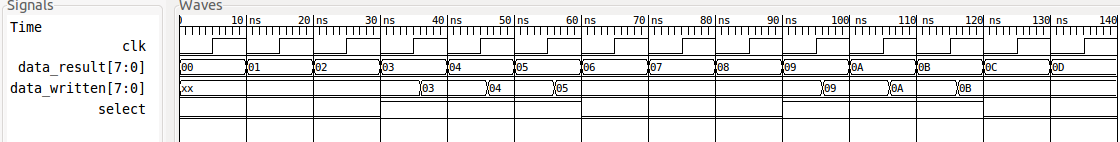
\includegraphics[scale=0.45]{../Codes/Verilog_Testbenches/scopes/Registers.png}
\label{fig:regs}
\end{figure}

\subsection{Banco de pruebas finales para el CPU}

Se realiz\' o una simulaci\' on de un conjunto de instrucciones variadas para el procesador, tratando de efectuar varios saltos incondicionales, tal como se puede observar en la Figura \ref{fig:jumps}.

\begin{figure}[hbtp]
\caption{Evaluaci\' on del m\' odulo CPU}
\centering
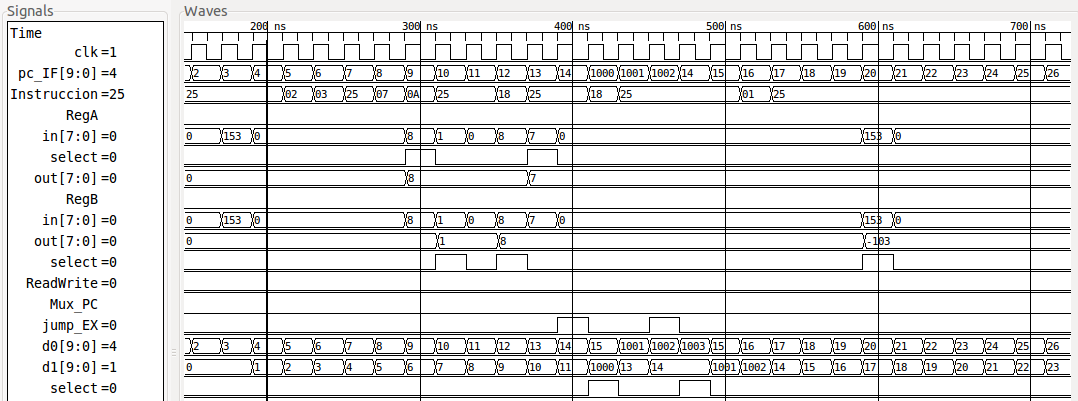
\includegraphics[scale=0.45]{../Codes/Verilog_Testbenches/scopes/Jump.png}
\label{fig:jumps}
\end{figure}

En la figura \ref{fig:jumps} se puede apreciar c\' omo en la posici\' on n\' umero 12 de la memoria se lee que se va a realizar un Jump (Instrucción 6'h18), y tres ciclos de reloj despu\' es el contador de programa realiza un salto a la posici\'on de memoria 1000. Esto muestra el correcto funcionamiento de los saltos de memoria absolutos (Jump). Adicionalmente en esta prueba, en la posici\' on 1000 se program\' o tambi\' en un Jump que regresara a las primeras posiciones de la memoria y continuar con la ejecuci\' on de las instrucciones en forma secuencial.

\paragraph{Instrucci\' on \textbf{SUBB}}
Para la implementaci\' on de la instrucci\' on \textbf{SUBB} se debe aclarar que en el procesador desarrollado la operaci\' on que ejecuta es \textit{B = A - B}. Esto se realiz\' o as\' i dado que se encontr\' o un error en la implementaci\; on pues se dise\~ no el caso para que fuera as\' i y no \textit{B = B - A}. Una posible soluci\' on futura para realizar la instrucci\' on tal y como se solicita es agregar una nueva salida al m\' odulo ALU que tenga el mismo resultado de la salida actual pero complementado, y luego agregar una se\~ nal de control al esquema que sea capaz de conocer si la instrucci\' on es \textit{SUBB}, debe tomar la segunda salida de la ALU, de lo contrario debe procesar la instrucci\' on con normalidad.




